\begin{center}

\includegraphics[width=0.3\textwidth]{content/3/chapter5/images/18.png}\\
Cippi在研究日历
\end{center}

\begin{tcolorbox}[breakable,enhanced jigsaw,colback=blue!5!white,colframe=blue!75!black,title={缺少编译器支持}]
	
截止到2020年底,还没有C++编译器支持chrono扩展。感谢HowardHinnant的原型库\href{https://github.com/HowardHinnant/date}{date},它本质上是C++20中时间功能扩展的超集,我用它做了一些实验。该库托管在GitHub上,使用date原型的方法有很多:

\begin{itemize}
\item 
可以在Wandbox上试试。Howard已经上传了date.h头文件,这足以使用新的类型std::time\_of\_day和日历。下面是Howard给出的链接:\href{https://wandbox.org/permlink/L8MwjzSSC3fXXrMd}{在Wandbox上试一试吧!}。

\item 
下载项目并构建它,GitHub上\href{https://github.com/HowardHinnant/date}{date}提供了更多信息。想要尝试新的时区特性时,需要进行此步骤。
\end{itemize}

本章的例子使用Howard Hinnant的库。不过,我的解释是基于C++20术语的。当C++编译器支持扩展的chrono功能时,我将使示例适配C++20的语法。
\end{tcolorbox}

\begin{itemize}
\item 
一天中的时间是指从午夜开始的时间长度,分为小时、分钟、秒和分秒。

\item 
Calendar表示各种日历日期,如年、月、工作日或一周的第n天。

\item 
时区表示特定于地理区域的时间。
\end{itemize}

时区功能(C++20)是基于日历功能(C++20),而日历功能(C++20)是基于时间功能(C++11)。


\begin{tcolorbox}[breakable,enhanced jigsaw,colback=blue!5!white,colframe=blue!75!black,title={C++11的时间库}]
	
为了充分利用本节的内容,必须先对chrono库有基本的了解。C++11引入了三个主要组件来处理时间:

\begin{itemize}
\item 
时间点由时间起点(即所谓的epoch)和时间段定义。

\item 
时间间隔由两个时间点之间的差值,使用时钟周期数表示。

\item 
时钟由时间起点(epoch)和时钟周期数组成,可以计算出当前的时间点。
\end{itemize}

老实说,时间对我来说是个谜。一方面,每个人对时间都有一个直观的概念;另一方面,正式定义它极具挑战性。例如,时间点(time point)、时间段(time duration)和时钟(clock)三者相互依赖。若想了解更多C++11中有关时间的功能,请阅读我在\href{https://www.modernescpp.com/index.php/tag/time}{time}上发布的关于时间的文章。
	
\end{tcolorbox}

\subsubsubsection{5.5.1\hspace{0.2cm}日期}

std::chrono::hh\_mm\_ss是自午夜开始的时间段,分为小时、分钟、秒和分秒,这种类型通常用作格式化工具。下表提供了std::chrono::hh\_mm\_ss实例tOfDay的简明概述。

\begin{center}
日期
\end{center}

\begin{table}[H]
\centering
\begin{tabular}{ll}
\textbf{函数}         & \textbf{描述}                        \\ \hline
tOfDay.hours()            & 返回从午夜开始累计的小时数   \\
tOfDay.minutes()          & 返回从午夜开始累计的分钟数 \\
tOfDay.seconds()          & 返回从午夜开始累计的秒数 \\
tOfDay.subseconds()       & 返回从午夜开始累计的分秒数  \\
tOfDay.to\_duration()     & 返回从午夜以来的时间段    \\
std::chrono::make12(hour) & 返回12小时的等价24小时的时间格式 \\
std::chrono::make24(hour) & 返回24小时的等价12小时的时间格式 \\
std::chrono::is\_am(hour) & 检测24小时时间格式是否为a.m.  \\
std::chrono::is\_pm(hour) & 检测24小时时间格式是否为p.m.
\end{tabular}
\end{table}

这些函数的使用起来很简单。

\begin{lstlisting}[style=styleCXX]
// timeOfDay.cpp

#include <chrono>
#include <iostream>

int main() {
	using namespace std::chrono;    
	
	using namespace std::chrono_literals;
	
	std::cout << std::boolalpha << '\n';
	auto timeOfDay = std::chrono::hh_mm_ss(10.5h + 98min + 2020s + 0.5s);
	
	std::cout<< "timeOfDay: " << timeOfDay << '\n';
	
	std::cout << '\n';
	
	std::cout << "timeOfDay.hours(): " << timeOfDay.hours() << '\n';
	std::cout << "timeOfDay.minutes(): " << timeOfDay.minutes() << '\n';
	std::cout << "timeOfDay.seconds(): " << timeOfDay.seconds() << '\n';
	std::cout << "timeOfDay.subseconds(): " << timeOfDay.subseconds() << '\n';
	std::cout << "timeOfDay.to_duration(): " << timeOfDay.to_duration() << '\n';
	std::cout << '\n';
	
	std::cout << "date::hh_mm_ss(45700.5s): " << std::chrono::hh_mm_ss(45700.5s) << '\n';
	
	std::cout << '\n';
	
	std::cout << "date::is_am(5h): " << std::chrono::is_am(5h) << '\n';
	std::cout << "date::is_am(15h): " << std::chrono::is_am(15h) << '\n';
	
	std::cout << '\n';
	
	std::cout << "date::make12(5h): " << std::chrono::make12(5h) << '\n';
	std::cout << "date::make12(15h): " << std::chrono::make12(15h) << '\n';
	
}
\end{lstlisting}

首先,我在第12行创建了std::chrono::hh\_mm\_ss: timeOfDay的一个新实例。C++14添加了chrono字面值,就可以添加一些时间时间段来初始化一天中的时间对象。使用C++20,可以直接输出timeOfDay(第14行),这就是在第7行中引入命名空间date的原因,其余部分应该很容易阅读。第18-21行,以小时、分钟、秒和分数秒为单位显示了从午夜开始的时间分量。第22行返回自午夜以来的时间时间段,以秒为单位。第26行更有趣:给定的秒对应于第15行中显示的时间。若给定的时间是a.m.,则返回第30和32行。第35行和36行返回与给定小时等价12小时的时间格式。

下面是程序的输出:

\begin{tcblisting}{commandshell={}}
timeOfDay: 12:41:40.500000

timeOfDay.hours(): 12h
timeOfDay.minutes(): 41min
timeOfDay.seconds(): 40s
timeOfDay.subseconds(): 0.500000s
timeOfDay.to_duration(): 45700.500000s

date::hh_mm_ss(45700.5s): 12:41:40.500000

date::is_am(5h): true
date::is_am(15h): false

date::make12(5h): 5h
date::make12(15h): 3h
\end{tcblisting}

\subsubsubsection{5.5.2\hspace{0.2cm}日历日期}

C++20中一个新的chrono扩展类型是日历日期。C++20支持多种方式来创建日历日期,并可与之交互。那什么是日历日期呢?

日历日期是由一年、一个月和一天组成的日期,所以C++20有一个特定的数据类型std::chrono::year\_month\_day。C++20提供了很多相关的功能。在下面的表中,将了解日历日期类型,然后再展示各种方式的用例。

\begin{center}
各种日历日期类型
\end{center}

\begin{table}[H]
\centering
\begin{tabular}{ll}
\textbf{类型}                 & \textbf{描述}                                   \\ \hline
std::chrono::last\_spec       & 一个月的最后一天或工作日           \\
std::chrono::day              & 一个月中的一天                            \\
std::chrono::month            & 一年中的一个月                           \\
std::chrono::year             & 表示公历中的一年            \\
std::chrono::weekday          & 表示公历中的一周中的一天 \\
std::chrono::weekday\_indexed & 表示每月的第n个工作日                 \\
std::chrono::weekday\_last    & 表示一个月的最后一个工作日                 \\
std::chrono::month\_day       & 表示特定月份中的特定日期          \\
std::chrono::month\_day\_last & 表示特定月份的最后一天            \\
std::chrono::month\_weekday   & 表示特定月份的第n个工作日        \\
std::chrono::month\_weekday\_last            & 表示特定月份的最后一个工作日           \\
std::chrono::year\_month      & 表示特定年份中的特定月份         \\
std::chrono::year\_month\_day & 表示特定的年、月和日             \\
std::chrono::year\_month\_day\_last          & 表示特定年份和月份的最后一天      \\
std::chrono::year\_month\_weekday            & 表示特定年份和月份的第n个工作日  \\
std::chrono::year\_month\_day\_weekday\_last & 表示特定年份和月份的最后一个工作日 \\
std::chrono::operator /       & 创建公历日期              
\end{tabular}
\end{table}

先创建几个日历日期。

\hspace*{\fill} \\ %插入空行
\noindent
\textbf{5.5.2.1\hspace{0.2cm}创建日历日期}

createCalendar.cpp展示了创建日历相关日期的各种方法。

\begin{lstlisting}[style=styleCXX]
// createCalendar.cpp

#include <iostream>
#include "date.h"

int main() {

	std::cout << '\n';
	
	using namespace date;
	
	constexpr auto yearMonthDay{year(1940)/month(6)/day(26)};
	std::cout << yearMonthDay << " ";
	std::cout << date::year_month_day(1940_y, June, 26_d) << '\n';
	
	std::cout << '\n';
	
	constexpr auto yearMonthDayLast{year(2010)/March/last};
	std::cout << yearMonthDayLast << " ";
	std::cout << date::year_month_day_last(2010_y, month_day_last(month(3))) << '\n';
	
	constexpr auto yearMonthWeekday{year(2020)/March/Thursday[2]};
	std::cout << yearMonthWeekday << " ";
	std::cout << date::year_month_weekday(2020_y, month(March), Thursday[2]) << '\n';
	
	constexpr auto yearMonthWeekdayLast{year(2010)/March/Monday[last]};
	std::cout << yearMonthWeekdayLast << " ";
	std::cout << date::year_month_weekday_last(2010_y, month(March),
	weekday_last(Monday)) << '\n';
	
	std::cout << '\n';
	
	constexpr auto day_{day(19)};
	std::cout << day_ << " ";
	std::cout << date::day(19) << '\n';
	
	constexpr auto month_{month(1)};
	std::cout << month_ << " ";
	std::cout << date::month(1) << '\n';
	
	constexpr auto year_{year(1988)};
	std::cout << year_ << " ";
	std::cout << date::year(1988) << '\n';
	
	constexpr auto weekday_{weekday(5)};
	std::cout << weekday_ << " ";
	std::cout << date::weekday(5) << '\n';
	
	constexpr auto yearMonth{year(1988)/1};
	std::cout << yearMonth << " ";
	std::cout << date::year_month(year(1988), January) << '\n';
	
	constexpr auto monthDay{10/day(22)};
	std::cout << monthDay << " ";
	std::cout << date::month_day(October, day(22)) << '\n';
	
	constexpr auto monthDayLast{June/last};
	std::cout << monthDayLast << " ";
	std::cout << date::month_day_last(month(6)) << '\n';
	
	constexpr auto monthWeekday{2/Monday[3]};
	std::cout << monthWeekday << " ";
	std::cout << date::month_weekday(February, Monday[3]) << '\n';
	
	constexpr auto monthWeekDayLast{June/Sunday[last]};
	std::cout << monthWeekDayLast << " ";
	std::cout << date::month_weekday_last(June, weekday_last(Sunday)) << '\n';
	
	std::cout << '\n';

}
\end{lstlisting}

有两种方法可以创建日历日期。可以使用yearMonthDay\{year(1940)/month(6)/day(26)\}(第12行),或直接使用显式类型date::year\_month\_day(1940y, June, 26d)(第14行)。使用显式类型非常有趣,因为其使用了日期-时间的字面值1940y、26d和常量June。这里,我把对第一种好用的语法的解释推迟到下一节。

第18行、第22行和第26行提供了更多创建日历日期的方法。

\begin{enumerate}
\item 
第18行:2010年3月的最后一天
\begin{lstlisting}[style=styleCXX]
{year(2010)/March/last}
\end{lstlisting}
或
\begin{lstlisting}[style=styleCXX]
year_month_day_last(2010y, month_day_last(month(3)))
\end{lstlisting}

\item 
第22行:2020年3月第二个星期四
\begin{lstlisting}[style=styleCXX]
{year(2020)/March/Thursday[2]}
\end{lstlisting}
或
\begin{lstlisting}[style=styleCXX]
year_month_weekday(2020y, month(March), Thursday[2])
\end{lstlisting}

\item 
第26行:2010年3月的最后一个星期一
\begin{lstlisting}[style=styleCXX]
{year(2010)/March/Monday[last]}
\end{lstlisting}
或
\begin{lstlisting}[style=styleCXX]
year_month_weekday_last(2010y, month(March), weekday_last(Monday))
\end{lstlisting}
\end{enumerate}

其余日历类型代表一天(第33行)、一个月(第37行)或一年(第41行)。可以将它们组合使用,并将其用作完全指定的日历日期的基本构建块,例如第18、22或26行。

这是程序的输出:

\begin{tcblisting}{commandshell={}}
1940-06-26 1940-06-26

2010/Mar/last 2021/Mar/last
2020/Mar/Thu[2] 2020/Mar/Thu[2]
2010/Mar/mon[last] 2010/Mar/mon[last]

19 19
Jan Jan
1988 1988
Fri Fri
1988/Jan 1988/Jan
Oct/22 Oct/22
Jun/last Jun/last
Feb/Mon[3] Feb/Mon[3]
Jun/Sun[last] Jun/Sun[last]
\end{tcblisting}

\hspace*{\fill} \\ %插入空行
\noindent
\textbf{5.5.2.2\hspace{0.2cm}“好用的”语法解释}

这种语法由重载除法运算符组成,用于指定日历日期。重载操作符支持时间字面量(例如:2020y, 31d)和常量(January, February, March, April, May, June, July, August, September, October, November, December)。

使用这种语法时,可以使用以下年、月和日的三种组合。

\begin{lstlisting}[style=styleCXX]
year/month/day
day/month/year
month/day/year
\end{lstlisting}

这些组合并不是随意选择的,是可以在世界范围内使用的。但不能使用其他的组合方式。

当为第一个参数选择类型年、月或日时,其余两个参数的类型就不再需要了,用数字就可以了。

\begin{lstlisting}[style=styleCXX]
// cuteSyntax.cpp

#include <iostream>
#include "date.h"

int main() {
	
	std::cout << '\n';
	
	using namespace date;
	
	constexpr auto yearMonthDay{year(1966)/6/26};
	std::cout << yearMonthDay << '\n';
	
	constexpr auto dayMonthYear{day(26)/6/1966};
	std::cout << dayMonthYear << '\n';
	
	constexpr auto monthDayYear{month(6)/26/1966};
	std::cout << monthDayYear << '\n';
	
	constexpr auto yearDayMonth{year(1966)/month(26)/6};
	std::cout << yearDayMonth << '\n';
	
	std::cout << '\n';

}
\end{lstlisting}

年/日/月的组合(第21行)是非法的,这会导致一条运行时的错误。

\begin{tcblisting}{commandshell={}}
1966-06-26
1966-06-26
1966-06-26
1966-26-06 is not a valid data
\end{tcblisting}

\begin{center}
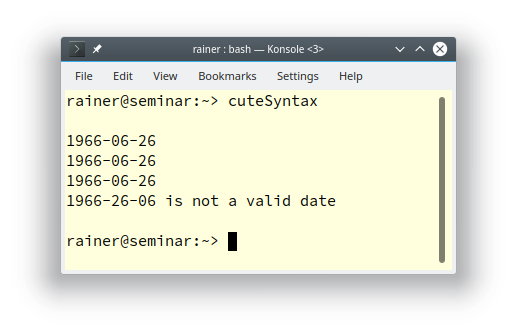
\includegraphics[width=0.6\textwidth]{content/3/chapter5/images/21.png}\\
\end{center}

这里,假设希望以可读的形式显示日历日期\{year(2010)/March/last\},例如2020-03-31。这是local\_days或sys\_days操作符的任务。

\hspace*{\fill} \\ %插入空行
\noindent
\textbf{5.5.2.3\hspace{0.2cm}显示日历日期}

使用std::chrono::local\_days或std::chrono::sys\_days,可以将日历日期转换为std::chrono::time\_point。例子中,我使用的是std::chrono::sys\_days,其基于\href{https://en.cppreference.com/w/cpp/chrono/system_clock}{std::chrono::system\_clock}。这里,我将对前一个程序createCalendar.cpp中的日历日期进行转换(第18、22和26行)。

\begin{lstlisting}[style=styleCXX]
// sysDays.cpp

#include <iostream>
#include "date.h"

int main() {

	std::cout << '\n';
	
	using namespace date;
	
	constexpr auto yearMonthDayLast{year(2010)/March/last};
	std::cout << "sys_days(yearMonthDayLast): "
	<< sys_days(yearMonthDayLast) << '\n';
	
	constexpr auto yearMonthWeekday{year(2020)/March/Thursday[2]};
	std::cout << "sys_days(yearMonthWeekday): "
	<< sys_days(yearMonthWeekday) << '\n';
	
	constexpr auto yearMonthWeekdayLast{year(2010)/March/Monday[last]};
	std::cout << "sys_days(yearMonthWeekdayLast): "
	<< sys_days(yearMonthWeekdayLast) << '\n';
	
	std::cout << '\n';
	
	constexpr auto leapDate{year(2012)/February/last};
	std::cout << "sys_days(leapDate): " << sys_days(leapDate) << '\n';
	
	constexpr auto noLeapDate{year(2013)/February/last};
	std::cout << "sys_day(noLeapDate): " << sys_days(noLeapDate) << '\n';
	
	std::cout << '\n';

}
\end{lstlisting}

std::chrono::last常量(第11行)让可以轻松确定一个月有多少天。输出显示,2012是闰年(第26行),而2013年不是(第29行)。

\begin{tcblisting}{commandshell={}}
sys_days(yearMonthDayLast): 2010-03-31
sys_days(yearMonthWeekday): 2020-03-12
sys_days(yearMonthWeekdayLast): 2010-03-29

sys_days(leapDate): 2012-02-29
sys_days(noLeapDate): 2013-02-28
\end{tcblisting}

假设有一个日历日期,例如:year(2100)/2/29。第一个问题是:这个日期有效吗?

\hspace*{\fill} \\ %插入空行
\noindent
\textbf{5.5.2.4\hspace{0.2cm}检查日期是否有效}

C++20中的各种日历类型都有一个ok函数。若日期有效,该函数返回true。

\begin{lstlisting}[style=styleCXX]
// leapYear.cpp

#include <iostream>
#include <chrono>

int main() {
	
	std::cout << std::boolalpha << '\n';
	
	using namespace std::chrono;
	
	std::cout << "Valid days" << '\n';
	day day31(31);
	day day32 = day31 + days(1);
	std::cout << " day31: " << static_cast<unsigned>(day31) << "; ";
	std::cout << "day31.ok(): " << day31.ok() << '\n';
	std::cout << " day32: " << static_cast<unsigned>(day32) << "; ";
	std::cout << "day32.ok(): " << day32.ok() << '\n';
	
	
	std::cout << '\n';
	
	std::cout << "Valid months" << '\n';
	month month1(1);
	month month0(0);
	std::cout << " month1: " << static_cast<unsigned>(month1) << "; ";
	std::cout << "month1.ok(): " << month1.ok() << '\n';
	std::cout << " month0: " << static_cast<unsigned>(month0) << "; ";
	std::cout << "month0.ok(): " << month0.ok() << '\n';
	
	std::cout << '\n';
	
	std::cout << "Valid years" << '\n';
	year year2020(2020);
	year year32768(-32768);
	std::cout << " year2020: " << static_cast<int>(year2020) << "; ";
	std::cout << "year2020.ok(): " << year2020.ok() << '\n';
	std::cout << " year32768: " << static_cast<int>(year32768) << "; ";
	std::cout << "year32768.ok(): " << year32768.ok() << '\n';
	
	std::cout << '\n';
	
	std::cout << "Leap Years" << '\n';
	
	constexpr auto leapYear2016{year(2016)/2/29};
	constexpr auto leapYear2020{year(2020)/2/29};
	constexpr auto leapYear2024{year(2024)/2/29};
	
	std::cout << " leapYear2016.ok(): " << leapYear2016.ok() << '\n';
	std::cout << " leapYear2020.ok(): " << leapYear2020.ok() << '\n';
	std::cout << " leapYear2024.ok(): " << leapYear2024.ok() << '\n';
	
	std::cout << '\n';
	
	std::cout << "No Leap Years" << '\n';
	
	constexpr auto leapYear2100{year(2100)/2/29};
	constexpr auto leapYear2200{year(2200)/2/29};
	constexpr auto leapYear2300{year(2300)/2/29};
	
	std::cout << " leapYear2100.ok(): " << leapYear2100.ok() << '\n';
	std::cout << " leapYear2200.ok(): " << leapYear2200.ok() << '\n';
	std::cout << " leapYear2300.ok(): " << leapYear2300.ok() << '\n';
	
	std::cout << '\n';
	
	std::cout << "Leap Years" << '\n';
	
	constexpr auto leapYear2000{year(2000)/2/29};
	constexpr auto leapYear2400{year(2400)/2/29};
	constexpr auto leapYear2800{year(2800)/2/29};
	
	std::cout << " leapYear2000.ok(): " << leapYear2000.ok() << '\n';
	std::cout << " leapYear2400.ok(): " << leapYear2400.ok() << '\n';
	std::cout << " leapYear2800.ok(): " << leapYear2800.ok() << '\n';
	
	std::cout << '\n';
	
}
\end{lstlisting}

程序中检查给定的日期(第12行)、给定的月份(第23行)或给定的年份(第33行)是否有效。天的范围是[1,31],月的范围是[1,12],年的范围是[-32767,32767],所以ok()将返回false。当我显示不同的值时,若值无效,则输出显示:“不是有效的日期”、“不是有效的月份”、“不是有效的年份”[译者注:标准库不会输出这些信息]。其次,月份值会以字符串形式显示。

\begin{tcblisting}{commandshell={}}
Valid days
  day31: 31; day31.ok(): true
  day32: 32; day32.ok(): false

Valid months
  month1: 1; month1.ok(): true
  month0: 0; month0.ok(): false

Valid years
  year2020: 2020; year2020.ok(): true
  year32768: -32768; year32768.ok(): false

Leap Years
  leapYear2016.ok(): true
  leapYear2020.ok(): true
  leapYear2024.ok(): true

No Leap Years
  leapYear2100.ok(): false
  leapYear2200.ok(): false
  leapYear2300.ok(): false

Leap Years
  leapYear2000.ok(): true
  leapYear2400.ok(): true
  leapYear2800.ok(): true
\end{tcblisting}

可以在日历日期上使用ok,所以检查一个特定的日历日期是否为闰日就很容易了,从而就可以判断相应的年份是否为闰年。全球使用的\href{https://en.wikipedia.org/wiki/Gregorian_calendar}{格里高利历}中,适用以下规则:

非整世纪年能能被4整除的年份是闰年。
 
整世纪年能被100整除的年份是不是闰年,能被400整除的年份才是闰年。

有点复杂哈?leapYears.cpp用代码表达了这个规则。

扩展的chrono库可以很容易地计算日历日期之间的时间时间段。

\hspace*{\fill} \\ %插入空行
\noindent
\textbf{5.5.2.5\hspace{0.2cm}查询日历日期}

下面的queryCalendarDates.cpp就是在查询一些日历日期。

\begin{lstlisting}[style=styleCXX]
// queryCalendarDates.cpp

#include "date.h"
#include <iostream>

int main() {
	
	using namespace date;
	
	std::cout << '\n';
	
	auto now = std::chrono::system_clock::now();
	std::cout << "The current time is: " << now << " UTC\n";
	std::cout << "The current date is: " << floor<days>(now) << '\n';
	std::cout << "The current date is: " << year_month_day{floor<days>(now)}
	<< '\n';
	std::cout << "The current date is: " << year_month_weekday{floor<days>(now)}
	<< '\n';
	
	std::cout << '\n';
	
	
	auto currentDate = year_month_day(floor<days>(now));
	auto currentYear = currentDate.year();
	std::cout << "The current year is " << currentYear << '\n';
	auto currentMonth = currentDate.month();
	std::cout << "The current month is " << currentMonth << '\n';
	auto currentDay = currentDate.day();
	std::cout << "The current day is " << currentDay << '\n';
	
	std::cout << '\n';
	
	auto hAfter = floor<std::chrono::hours>(now) - sys_days(January/1/currentYear);
	std::cout << "It has been " << hAfter << " since New Year!\n";
	
	auto nextYear = currentDate.year() + years(1);
	auto nextNewYear = sys_days(January/1/nextYear);
	auto hBefore = sys_days(January/1/nextYear) - floor<std::chrono::hours>(now);
	std::cout << "It is " << hBefore << " before New Year!\n";
	
	std::cout << '\n';
	
	std::cout << "It has been " << floor<days>(hAfter) << " since New Year!\n";
	std::cout << "It is " << floor<days>(hBefore) << " before New Year!\n";
	
	std::cout << '\n';
	
}
\end{lstlisting}

使用C++20扩展,可以直接显示时间点,例如:now(第12行)。atd::chrono::floor将时间点转换为atd::chrono::sys\_days,这个值可以用来初始化日历类型std::chrono::year\_month\_day。将值放入std::chrono::year\_month\_weekday日历类型中时,得到的答案是这个特定的日子是10月的第3个星期二。当然,还可以基于月份计算日历日期,例如当前的年、月或日(第23行)。

第33行是最有趣的一行。当使用基于小时的日期,从当前日期减去当前年份的1月1日时,得到了自新的一年以来的小时数。相反,当从明年的1月1日减去当前日期(第37行)时,使用小时解析后,得到了到新的一年的小时数(也许你不喜欢基于小时的方式,第42和43行使用基于天的方式显示值)。

\begin{tcblisting}{commandshell={}}
The current time is: 2020-10-20 06:08:01.516990636 UTC
The current date is: 2020-10-20
The current date is: 2020-10-20
The current data is: 2020/Oct/Tue[3]

The current year is 2020
The current month is Oct
The current day is 20

It has been 7038h sine New Year!
It is 1746h before New Year!

It has been 293d since New Year!
It is 72d before New Year!
\end{tcblisting}

现在,我想知道我的生日是星期几。

\hspace*{\fill} \\ %插入空行
\noindent
\textbf{5.5.2.6\hspace{0.2cm}查询星期几}

由于扩展的chrono库,可以很容易地获得给定日历日期是星期几。

\begin{lstlisting}[style=styleCXX]
// weekdaysOfBirthdays.cpp

#include <cstdlib>
#include <iostream>
#include "date.h"

int main() {
	
	std::cout << '\n';
	
	using namespace date;
	
	int y;
	int m;
	int d;
	
	std::cout << "Year: ";
	std::cin >> y;
	std::cout << "Month: ";
	std::cin >> m;
	std::cout << "Day: ";
	std::cin >> d;
	
	std::cout << '\n';
	
	auto birthday = year(y)/month(m)/day(d);
	
	if (not birthday.ok()) {
		std::cout << birthday << '\n';
		std::exit(EXIT_FAILURE);
	}
	
	std::cout << "Birthday: " << birthday << '\n';
	auto birthdayWeekday = year_month_weekday(birthday);
	std::cout << "Weekday of birthday: " << birthdayWeekday.weekday() << '\n';
	
	auto currentDate = year_month_day(floor<days>(
	std::chrono::system_clock::now()));
	auto currentYear = currentDate.year();
	
	auto age = (int)currentDate.year() - (int)birthday.year();
	std::cout << "Your age: " << age << '\n';
	
	std::cout << '\n';
	
	std::cout << "Weekdays for your next 10 birthdays" << '\n';
	
	for (int i = 1, newYear = (int)currentYear; i <= 10; ++i ) {
		std::cout << " Age " << ++age << '\n';
		auto newBirthday = year(++newYear)/month(m)/day(d);
		std::cout << " Birthday: " << newBirthday << '\n';
		std::cout << " Weekday of birthday: "
				  << year_month_weekday(newBirthday).weekday() << '\n';
	}
	
	std::cout << '\n';
	
}
\end{lstlisting}

首先,程序询问我的出生的年、月和日(第17行)信息。根据输入,创建一个日历日期(第26行)并检查它是否有效(第28行)。现在,显示了生日的星期名称。我使用日历日期来填充std::chrono::year\_month\_weekday(第34行)。为了获得日历类型year的int表示形式,必须将其转换为int(第41行)。现在,可以显示年龄了。最后,for循环为接下来的十个生日(第46行)显示以下信息:年龄、日历日期和工作日。这里,只需要增加age和newYear就好。

以我生日作为输入时,程序运行的后的输出。

\begin{tcblisting}{commandshell={}}
Year: 1966
Month: 6
Day: 26

Birthday: 1966-06-26
Weekday of birthday: Sun
Your age: 57

Weekdays for your next 10 birthdays
  Age 58
    Birthday: 2024-06-26
    Weekday of birthday: Wed
  Age 59
    Birthday: 2025-06-26
    Weekday of birthday: Thu
  Age 60
    Birthday: 2026-06-26
    Weekday of birthday: Fri
  Age 61
    Birthday: 2027-06-26
    Weekday of birthday: Sat
  Age 62
    Birthday: 2028-06-26
    Weekday of birthday: Mon
  Age 63
    Birthday: 2029-06-26
    Weekday of birthday: Tue
  Age 64
    Birthday: 2030-06-26
    Weekday of birthday: Wed
  Age 65
    Birthday: 2031-06-26
    Weekday of birthday: Thu
  Age 66
    Birthday: 2032-06-26
    Weekday of birthday: Sat
  Age 67
    Birthday: 2033-06-26
    Weekday of birthday: Sun
\end{tcblisting}

\begin{center}
我生日那天的星期名称
\end{center}

\hspace*{\fill} \\ %插入空行
\noindent
\textbf{5.5.2.7\hspace{0.2cm}计算日期序数}

这是最后一个日历功能的例子,我想介绍HowardHinnant提供的\href{https://github.com/HowardHinnant/date/wiki/Examples-and-Recipes}{示例},其中有大约40个计时功能的示例。据推测,C++20中的chrono扩展并不容易获得,这么些示例就显得尤为宝贵了。读者们应该尝试这些例子,并将其作为进一步实验的起点,从而加强对这块内容的理解。

这里,介绍一个由\href{https://github.com/rbock}{Roland Bock}编写的计算日期顺序的程序。

“日期序数由一年和该年中的某一天组成(1月1日是第1天,12月31日是第365天或第366天)。年份可以直接从year\_month\_day获取。计算起来非常简单。在下面的代码中,我们知道year\_month\_day可以处理像1月0日这样的无效日期:”我在Roland(Roland Bock)的程序中添加了必要的头文件。

\begin{lstlisting}[style=styleCXX]
// ordinalDate.cpp

#include <chrono>
#include <iomanip>
#include <iostream>
#include <cassert>

int main()
{
	using namespace std::chrono;
	
	const auto time = std::chrono::system_clock::now();
	const auto daypoint = floor<days>(time);
	const auto ymd = year_month_day{daypoint};
	
	// calculating the year and the day of the year
	const auto year = ymd.year();
	const auto year_day = daypoint - sys_days{year/January/0};
	
	std::cout << (int)year << '-' << std::setfill('0') << std::setw(3)
	<< year_day.count() << '\n';
	
	// inverse calculation and check
	assert(ymd == year_month_day{sys_days{year/January/0} + year_day});
}
\end{lstlisting}

第13行截断当前时间点,该值在下一行中用于初始化日历日期。第18行计算两个时间点之间的时间时间段。两个时间点都以天为单位。最后,第21行中的year\_day.count()返回以天为单位的时间时间段。[译者注:输出表示该日为2020年的第298天]

\begin{tcblisting}{commandshell={}}
2020-298
\end{tcblisting}

\subsubsubsection{5.5.3\hspace{0.2cm}时区}

时区是一个地区,具有日期全部的历史,如夏令时或闰秒。C++20中的时区库是\href{https://www.iana.org/timezones}{IANA时区数据库}的完整解析器。下表将带您初步了解添加的新功能。

\begin{table}[H]
\centering
\begin{tabular}{ll}
\textbf{类型}                         & \textbf{时区数据类型描述}                                              \\ \hline
std::chrono::tzdb                     & 描述IANA时区数据库的副本                   \\ \hline
std::chrono::tdzb\_list               & 表示tzdb链表                              \\ \hline
\begin{tabular}[c]{@{}l@{}}std::chrono::get\_tzdb \\ std::chrono::get\_tzdb\_list \\ std::chrono::reload\_tzdb \\ std::chrono::remote\_version\end{tabular} &
访问和控制全局时区数据库 \\ \hline
std::chrono::locate\_zone             & 根据名称定位时区                           \\ \hline
std::chrono::current\_zone            & 返回当前时区                                     \\ \hline
std::chrono::time\_zone               & 表示时区                                            \\ \hline
std::chrono::sys\_info                & 表示特定时间点上的时区信息 \\ \hline
std::chrono::local\_info              & 表示本地时间到UNIX时间转换的信息 \\ \hline
std::chrono::zoned\_traits            & 用于表示时区的类指针                                      \\ \hline
std::chrono::zoned\_time              & 表示时区和时间点                           \\ \hline
std::chrono::leap\_second             & 包含有关闰秒的信息                \\ \hline
std::chrono::time\_zone\_link         & 表示时区的别名                    \\ \hline
std::chrono::nonexistent\_local\_time & 若本地时间不存在将引发该异常         \\ \hline
\end{tabular}
\end{table}

例子中,使用了std::chrono::zones\_time函数,其本质上是一个时区和一个时间点的组合。

\begin{tcolorbox}[breakable,enhanced jigsaw,colback=blue!5!white,colframe=blue!75!black,title={编译示例}]
	
要使用时区库编译程序,必须从\href{https://github.com/HowardHinnant/date}{date}库编译tz.cpp文件,并将其链接到\href{https://curl. se/}{curl}库。curl库是获取当前\href{https://www.iana.org/timezones}{IANA时区数据库}所必需的。下面的g++编译命令应该能让你明白所有的事情:

\hspace*{\fill} \\ %插入空行
\noindent
\textbf{使用原型库日期进行编译}
\begin{tcblisting}{commandshell={}}
g++ localTime.cpp -I <Path to data/tz.h> tz.cpp -std=c++17 \
  -lcurl -o localTime
\end{tcblisting}

\end{tcolorbox}

第一个例子很简单,显示UTC时间和本地时间。

\hspace*{\fill} \\ %插入空行
\noindent
\textbf{5.5.3.1\hspace{0.2cm}UTC时间和本地时间}

\href{https://en.wikipedia.org/wiki/Coordinated_Universal_Time}{UTC时间或协调世界时}是世界范围内的主要时间标准。计算机使用\href{https://en.wikipedia.org/wiki/Unix_time}{Unix time},非常接近UTC。UNIX时间是从UNIX纪元开始的秒数。Unix纪元是UTC时间1970年1月1日00:00:00。

std::chrono::system\_clock::now()在程序中返回localTime.cpp的Unix时间。

\begin{lstlisting}[style=styleCXX]
// localTime.cpp

#include "date/tz.h"
#include <iostream>

int main() {

	std::cout << '\n';
	
	using namespace date;
	
	std::cout << "UTC time" << '\n';
	auto utcTime = std::chrono::system_clock::now();
	std::cout << " " << utcTime << '\n';
	std::cout << " " << date::floor<std::chrono::seconds>(utcTime) << '\n':
	
	std::cout << '\n';
	
	std::cout << "Local time" << '\n';
	auto localTime = date::make_zoned(date::current_zone(), utcTime);
	std::cout << " " << localTime << '\n';
	std::cout << " " << date::floor<std::chrono::seconds>(localTime.get_local_time())
	          << '\n';
	
	auto offset = localTime.get_info().offset;
	std::cout << " UTC offset: " << offset << '\n';

	std::cout << '\n';

}
\end{lstlisting}

从第12行开始的代码块获取当前时间点,将其截断为秒并显示它。调用make\_zoned(第20行)创建std::chrono::zoned\_time localTime,使用localTime.get\_local\_time()将存储的时间点作为本地时间返回,这个时间点也截断为秒。localTime(第25行)还可以用于获取关于时区的信息。本例中,我感兴趣的是UTC时间的偏移。

\begin{tcblisting}{commandshell={}}
UTC time
  2020-10-23 21:23:26.128743011
  2020-10-23 21:23:26
  
Local time
  2020-10-23 21:23:26.128743011 CEST
  2020-10-23 21:23:26
  UTC offset: 7200s
\end{tcblisting}

下面的例子回答了我在教授不同时区时的一个关键问题:应该什么时候开始线上课程?

\hspace*{\fill} \\ %插入空行
\noindent
\textbf{5.5.3.2\hspace{0.2cm}线上课程的不同时区}

onlineClass.cpp程序回答以下问题:当我在当地时间(德国)7小时、13小时或17小时开始线上课程时,在相应的时区是几点?

线上课程将于2021年2月1日开始,时长为4小时。由于夏令时,日历日期对于得到正确答案至关重要。

\begin{lstlisting}[style=styleCXX]
// onlineClass.cpp

#include "date/tz.h"
#include <algorithm>
#include <iomanip>
#include <iostream>

template <typename ZonedTime>
auto getMinutes(const ZonedTime& zonedTime) {
	return date::floor<std::chrono::minutes>(zonedTime.get_local_time());
}

void printStartEndTimes(const date::local_days& localDay,
						const std::chrono::hours& h,
						const std::chrono::hours& durationClass,
						const std::initializer_list<std::string>& timeZones ){
	
	date::zoned_time startDate{date::current_zone(), localDay + h};
	date::zoned_time endDate{date::current_zone(), localDay + h + durationClass};
	std::cout << "Local time: [" << getMinutes(startDate) << ", "
	<< getMinutes(endDate) << "]" << '\n';
	
	longestStringSize = std::max(timeZones, [](const std::string& a,
	const std::string& b) { return a.size() < b.size(); }).size();
	for (auto timeZone: timeZones) {
		std::cout << " " << std::setw(longestStringSize + 1) << std::left
		          << timeZone
		          << "[" << getMinutes(date::zoned_time(timeZone, startDate))
		          << ", " << getMinutes(date::zoned_time(timeZone, endDate))
		          << "]" << '\n';
		
	}
}

int main() {

	using namespace std::string_literals;
	using namespace std::chrono;
	
	std::cout << '\n';
	
	constexpr auto classDay{date::year(2021)/2/1};
	constexpr auto durationClass = 4h;
	auto timeZones = {"America/Los_Angeles"s, "America/Denver"s,
					  "America/New_York"s, "Europe/London"s,
					  "Europe/Minsk"s, "Europe/Moscow"s,
					  "Asia/Kolkata"s, "Asia/Novosibirsk"s,
					  "Asia/Singapore"s, "Australia/Perth"s,
					  "Australia/Sydney"s};
	
	for (auto startTime: {7h, 13h, 17h}) {
		printStartEndTimes(date::local_days{classDay}, startTime,
						   durationClass, timeZones);
		std::cout << '\n';
	}

}
\end{lstlisting}

深入getMinutes(第8行)和printStartEndTimes(第13行)函数之前,先来看看main函数。main函数定义上课的日期、上课的时间段和所有时区。最后,使用基于范围的for循环(第51行),遍历所有时间段的起始时间。因为printStartEndTimes函数(第13行)的帮助,所有必要的信息都显示出来了。

从第18行开始,通过将课程的开始时间和时间段添加到日历日期,来计算培训的startDate和endDate。这两个值都在函数getMinutes(第8行)的帮助下显示出来了。floor<std::chrono::minutes>(zonedTime.get\_local\_time())从std::chrono::zoned\_time中获取存储的时间点,并将值以分钟为单位表示。为了正确对齐程序的输出,第23行确定所有时区名称中最长的一个的大小。第25行遍历所有时区,并显示时区名称,以及每个时间段的开始和结束。一些地方的时间甚至都在0点(半夜)之后了。

\begin{center}
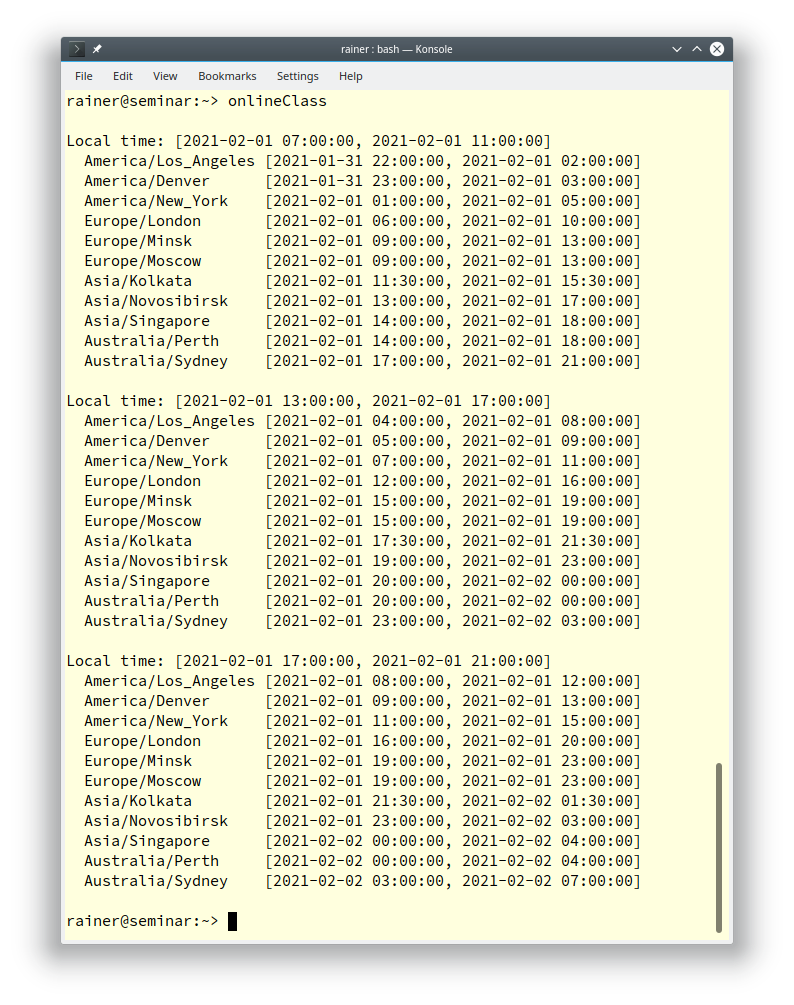
\includegraphics[width=0.55\textwidth]{content/3/chapter5/images/28.png}\\
\end{center}


\hspace*{\fill} \\ %插入空行
\noindent
\textbf{5.5.3.3\hspace{0.2cm}新时钟}

除了C++11中的墙壁时钟\href{https://www.modernescpp.com/index.php/the-three-clocks}{std::system\_clock}、稳定时钟std::steady\_clock和精确时钟std::high\_resolution\_clock之外,C++20还添加了5个时钟。

\begin{itemize}
\item 
std::utc\_clock: 协调世界时(UTC)的时钟。度量自UTC时间1970年1月1日00:00:00开始的时间,包括闰秒。

\item 
std::tai\_clock: \href{https://en.wikipedia.org/wiki/International_Atomic_Time}{国际原子时}(TAI)。测量1958年1月1日00:00:00以来的时间,并将该日期的UTC时间往前偏移10秒,不包括闰秒。

\item 
std::gps\_clock: GPS时间时钟,表示\href{https://en.wikipedia.org/wiki/Global_Positioning_System}{全球定位系统}(GPS)的时间。测量的是从1980年1月6日00:00:00 UTC开始的时间,不包括闰秒。

\item 
std::file\_clock: 文件时间时钟,是\href{https://en.cppreference.com/w/cpp/filesystem/file_time_type}{std::filesystem::file\_time\_type}的别名。

\item 
std::local\_t: 表示本地时间的伪时钟。
\end{itemize}


\hspace*{\fill} \\ %插入空行
\noindent
\textbf{5.5.3.4\hspace{0.2cm}时间的I/O}

格式化库中的std::chrono::parse函数和std::formatter函数,可以对chrono对象进行读写。

\begin{itemize}
\item 
std::chrono::parse: 从流中解析chrono对象。\href{https://en.cppreference.com/w/cpp/chrono/parse}{cppreference.com/parse}提供了关于格式字符串的详细信息。

\item 
std::formatter: 定义各种时间类型的特化。阅读关于std::formatter格式规范的详细信息,\href{https://en.cppreference.com/w/cpp/chrono/system_clock/formatter#Format_specification}{cppreference.com/formatter}。
\end{itemize}

\begin{tcolorbox}[breakable,enhanced jigsaw,colback=mygreen!5!white,colframe=mygreen!75!black,title={总结}]

\begin{itemize}
\item 
C++20在chrono库中添加了新的组件:当日时间、日历时间和时区。

\item 
当日时间是指从午夜开始的时间长度,分为小时、分钟、秒和分秒。

\item 
日历表示各种日历日期,如年、月、工作日或一周的第n天。

\item 
时区表示特定于地理区域的时间。
\end{itemize}

\end{tcolorbox}

\newpage






